%\graphicspath{{/Users/emiliendurif/Documents/prepa/sujets/DS/canne_robotise/}}


\question{A partir des données présentées dans la partie précédente compléter la chaine fonctionnelle relative à l'autofocus d'un appareil photo réflex.}

\ifthenelse{\boolean{corrige}}{
\begin{center}
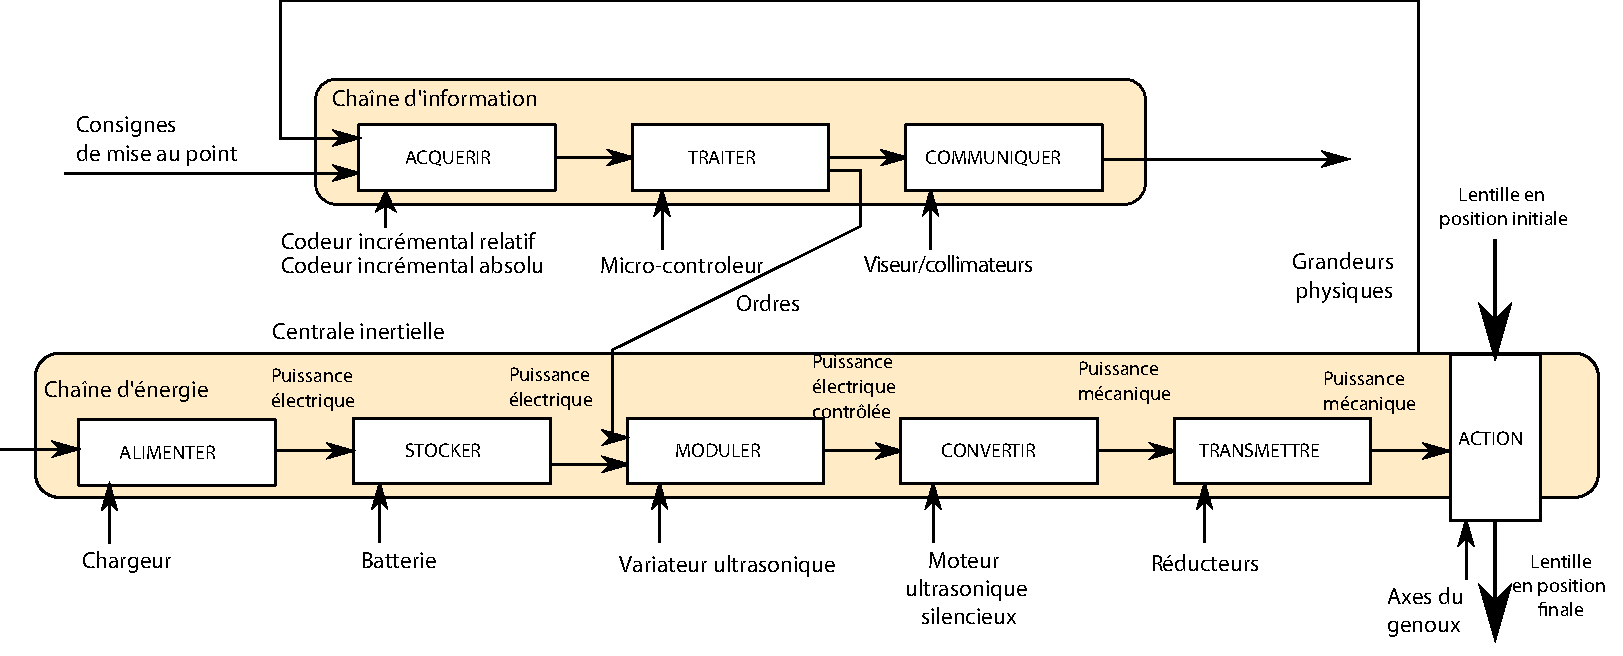
\includegraphics[width=1.0\textwidth]{images/chaine_fonctionnelle_corrige.pdf}
\end{center}
}
{
\begin{center}
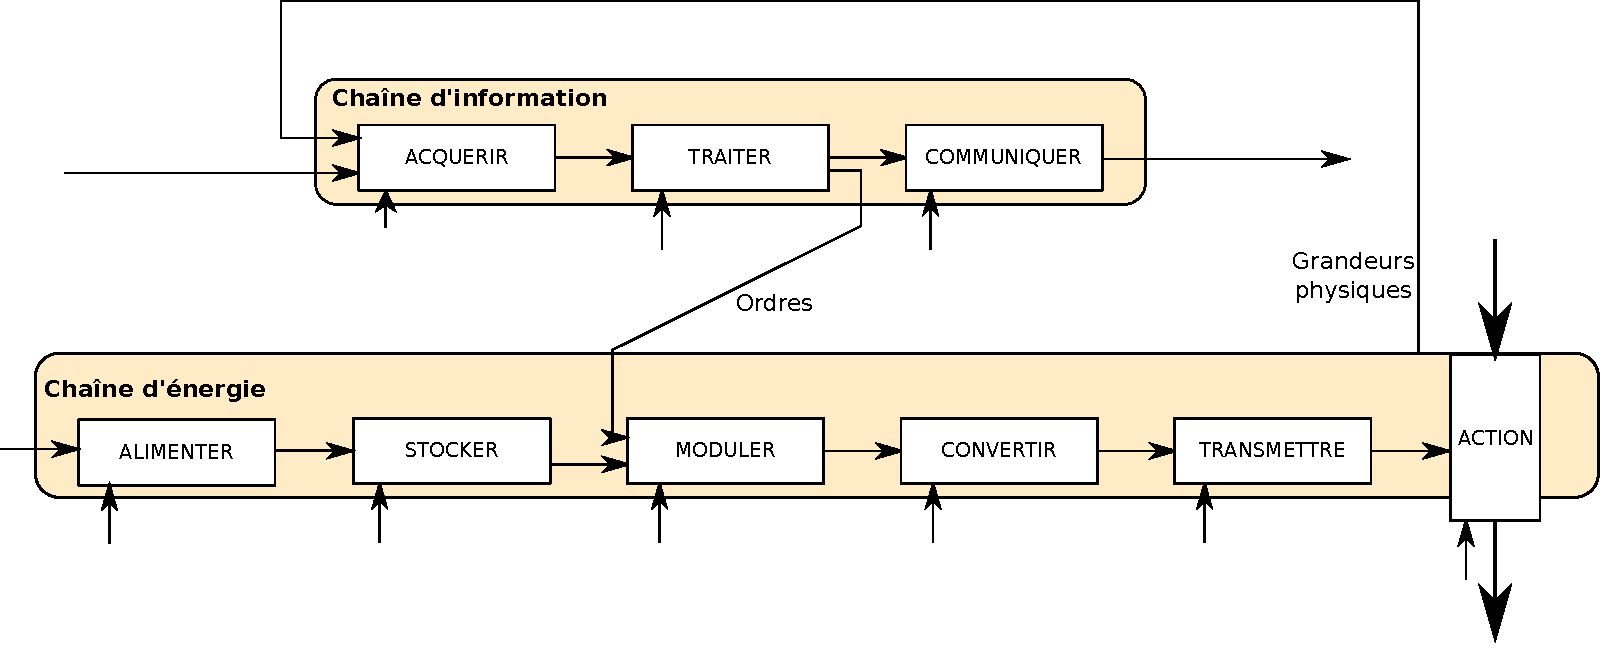
\includegraphics[width=1.0\textwidth]{images/chaine_fonctionnelle_0.pdf}
\end{center}
}

\question{Sur la modélisation multiphysique, repérer les parties acausales et les parties causales. Pour cela on surlignera en rouge ce qui représente la modélisation causale et en bleu ce qui représente la modélisation acausale.}

\ifthenelse{\boolean{corrige}}{
\begin{center}
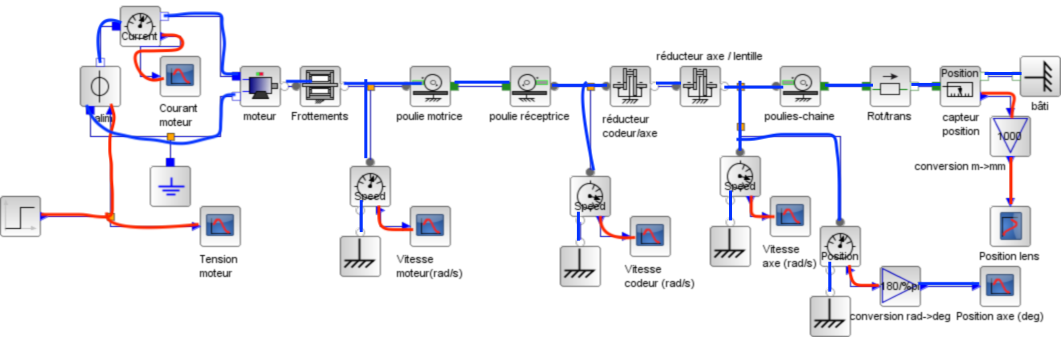
\includegraphics[width=1.0\textwidth]{images/image13_corrige.png}
\end{center}
}
{
\begin{center}
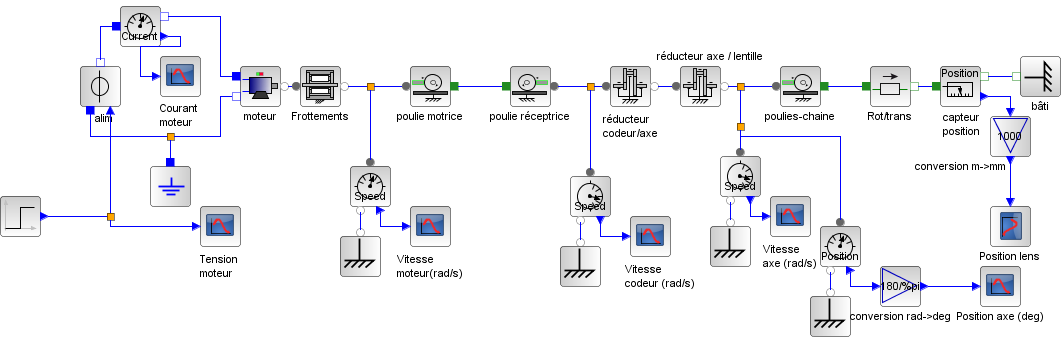
\includegraphics[width=1.0\textwidth]{images/image13.png}
\end{center}
}

\question{Décrire en quelques phrases ce modèle et ce qu'il permet de représenter. En particulier en explicitera les grandeur physiques et la façon dont elles sont mesurées. On précisera également qu'elles sont les grandeurs imposées et mesurées.}


\begin{texteCache}
La partie gauche du modèle représente le fonctionnement du moteur. Ce modèle permet de représenter la partie électrique. L'ensemble de la chaine d'énergie à partir du bloc "convertir" est représenté : poulie-courroie, réducteur, pouli-chaine, mécanisme de transformation de mouvement rotation/translation. Pour la partie électrique on impose une tension d'alimentation du moteur. On mesure en série le courant moteur. Le modèle permet de mesurer le long de la chaine d'énergie les grandeurs cinématique (rotations et translation) à chaque fois par rapport au bâti.
\end{texteCache}

\question{Préciser les différences du point de vue de l'utilisation entre les codeurs absolus et relatifs.}

\begin{texteCache}
\begin{itemize}
\item Un codeur absolu permet de connaître une position absolu. Un seule combinaison numérique correspond à une seul position. Ainsi à la mise à l'énergie la position est connu. Il n'y a donc pas besoin de calibrer le capteur.
\item Un codeur relatif permet de connaître une position relativement à la position de initiale. Ainsi à la mise à l'énergie la position n'est pas connu. Il est nécessaire de calibrer le capteur. Pour cela il faut que sur l'axe mesuré il y ait un dispositif de détection de butée mécanique ou électrique.
\end{itemize}
\end{texteCache}


\question{Donner la résolution possible pour la course totale de la
lentille mobile avec le codeur absolu. Justifier que le codeur absolu ne
soit utilisé que lors de la phase d'initialisation de l'objectif
photographique.}

\begin{texteCache}
Soit \(q\) la résolution du codeur absolu linéaire sur 4 bits et soit \(c\) la course totale de la lentille. On a~:

\[q_{\text{abs}} = \frac{c}{2^{4}}= \frac{6mm}{2^{4}} = 375\mu m\]

Comme \(q > 100\mu m\), la résolution est insuffisante pour une
utilisation normale.

\end{texteCache}


\question{Déterminer la relation entre le déplacement de la lentille mobile $d_l$ et la position angulaire du codeur incrémental $\theta_{rc}$. En déduire la résolution possible pour la course totale de
la lentille, si elle est déterminée en comptant les impulsions du codeur
incrémental sur les fronts montants.}

\begin{texteCache}

On commence par calculer le rapport de réduction du train simple
  d'engrenages avec en entrée \(\Delta\theta_{\text{rc}}\) la rotation
  de l'arbre du codeur incrémental et en sortie \(\Delta\theta_{l}\) la
  rotation de l'arbre de la lentille~:

\[{\frac{\Delta\theta_{l}}{\Delta\theta_{\text{rc}}} = \left( - 1 \right)^{7}\frac{Z_{3} \cdot Z_{4} \cdot Z_{5} \cdot Z_{7} \cdot Z_{9} \cdot Z_{11} \cdot Z_{12} \cdot Z_{14}}{Z_{4} \cdot Z_{5} \cdot Z_{6} \cdot Z_{8} \cdot Z_{10} \cdot Z_{12} \cdot Z_{13} \cdot Z_{15}} = r}\]\[{r = - \frac{Z_{3} \cdot Z_{7} \cdot Z_{9} \cdot Z_{11} \cdot Z_{14}}{Z_{6} \cdot Z_{8} \cdot Z_{10} \cdot Z_{13} \cdot Z_{15}} = 0,005}\]

Par définition du pas de la liaison hélicoïdale, on peut aussi écrire~:

\[d_{l} = \left| \frac{p}{2\pi}\Delta\theta_{l} \right| = \frac{p}{2\pi} \cdot r \cdot \Delta\theta_{\text{rc}}\]

La résolution en utilisant le codeur incrémental est donnée lorsque
l'arbre du codeur fait un angle de \(2\pi/30\). Cela s'écrit~:

\[q_{\text{inc}} = \frac{p}{2\pi} \cdot r \cdot \frac{2\pi}{30} = 5,2\mu m\]

\end{texteCache}




\question{En déduire le nombre de bits nécessaires pour coder
l'information « déplacement de la lentille mobile », si cette dernière
est donnée par le comptage du nombre d'impulsions au niveau du codeur
incrémental.}

\begin{texteCache}

Soit \(n\mathbb{\in N}\) le nombre de bits nécessaires pour coder l'information du codeur incrémental~:


\[{q_{\text{inc}} \geq \frac{c}{2^{n}}}\]

\[{2^{n} \geq \frac{c}{q_{\text{inc}}}}\]

\[{n \geq \frac{\ln\left( \frac{c}{q_{\text{inc}}} \right)}{\ln 2}}\]

\[{n \geq 10,23}\]


\end{texteCache}

\question{Passer les équations du modèle de connaissance dans le domaine de Laplace.}

\begin{texteCache}

\begin{align*}
C_m(p)-C_0(p)-f\cdotp\cdot  \Omega_m(p)=J\cdot p\cdot d\Omega_m(p)\\
\\
U_m(p)=E(p)+L_m\cdot p I_m(p)+R_m\cdot I_m(p)\\
\\
E(p)=K_e\cdot \Omega_m(p)\\
\\
C_m(p)=K_T\cdot I_m(p).
\end{align*}

\end{texteCache}

\question{On donne la structure du schéma bloc modélisant le moteur à courant continu. Compléter le schéma en précisant les fonctions de transfert et les variables.}

\ifthenelse{\boolean{corrige}}
{
\begin{center}
\begin{large}
\begin{tikzpicture}
\sbEntree{E0}
\sbComp[4]{c2}{E0}
\sbRelier[$U_m(p)$]{E0}{c2}
\sbBloc[1]{b2}{$\dfrac{1}{R_m+L_m\cdot p}$}{c2}
\sbRelier{c2}{b2}
\sbBloc[4]{b3}{$K_T$}{b2}
\sbRelier[$I_m(p)$]{b2}{b3}
%\sbComp[4]{c3}{b3}
\sbComph[6]{c3}{b3}
\sbDecaleNoeudy[-4]{c3}{E2}
\sbRelier[$C_0(p)$]{E2}{c3}
\sbBloc[7]{b4}{$\dfrac{1}{J\cdot p+f}$}{b3}
\sbRelier[$C_m(p)$]{b3}{c3}
\sbRelier{c3}{b4}
\sbSortie[5]{S}{b4}
\sbRelier[\hspace{.75cm}$\Omega_m(p)$]{b4}{S}
\sbDecaleNoeudy[4]{S}{v}
\sbBlocr[6]{b5}{$K_e$}{v}
\sbRelieryx{b4-S}{b5}
\sbRelierxy[$E(p)$]{b5}{c2}
\end{tikzpicture}
\end{large}
\end{center}
}
{
\begin{center}
\begin{large}
\begin{tikzpicture}
\sbEntree{E0}
\sbComp[4]{c2}{E0}
\sbRelier[$U_m(p)$]{E0}{c2}
\sbBloc[1]{b2}{}{c2}
\sbRelier{c2}{b2}
\sbBloc[4]{b3}{}{b2}
\sbRelier[]{b2}{b3}
%\sbComp[4]{c3}{b3}
\sbComph[6]{c3}{b3}
\sbDecaleNoeudy[-4]{c3}{E2}
\sbRelier[]{E2}{c3}
\sbBloc[7]{b4}{}{b3}
\sbRelier[]{b3}{c3}
\sbRelier{c3}{b4}
\sbSortie[5]{S}{b4}
\sbRelier[\hspace{.75cm}$\Omega_m(p)$]{b4}{S}
\sbDecaleNoeudy[4]{S}{v}
\sbBlocr[6]{b5}{}{v}
\sbRelieryx{b4-S}{b5}
\sbRelierxy[]{b5}{c2}
\end{tikzpicture}
\end{large}
\end{center}

}

\question{Exprimer sous ces conditions $I_m(p)$ en fonction de $U_m(p)$.}

\begin{texteCache}
Le rotor est bloqué, ainsi $\Omega_m(p)=0\rightarrow E(p)=0$.

On obtient alors,

\begin{align*}
I_m(p)=\dfrac{1}{R_m+L_m\cdot p}U_m(p).
\end{align*}



\end{texteCache}



\question{Donner l'expression de $U_m(p)$ et en déduire $I_m(p)$.}

\begin{texteCache}
D'après l'essai on peut approximer $u_m(t)$ à un échelon retardé de $T=50\mu s$ et d'amplitude $U_0=1,6V$.
Le théorème du retarde donne : 

\begin{align*}
U_m(p)=\dfrac{U_0e^{-T\cdot p}}{p}
\end{align*}

On en déduit : 

\begin{align*}
I_m(p)=\dfrac{U_0e^{-T\cdot p}}{p}\dfrac{1}{R_m+L_m\cdot p}
\end{align*}


\end{texteCache}

\question{A l'aide de la figure \ref{fig9} et des résultats précédents, justifier la forme de la courbe à partir du modèle proposé.}

\begin{texteCache}
D'après la question précédente on doit s'attendre à ce que $I_m(p)$ corresponde à la réponse indicielle retardé d'un premier ordre. Cela semble être le cas car on n'observe pas de dépassement et la courbe présente une tangente à l'origine de l'échelon ($t=T$) non nulle.

\end{texteCache}

\question{Déterminer la résistance d'induit $R_m$ et de l'inductance d'induit $L_m$ à partir de l'essai à rotor bloqué et des équations précédentes.}

\begin{texteCache}
Avec \(u_{m} = u_{m0} = 1,6V = cst\). La courbe de \(i_{m}(t)\)
représente donc la réponse d'un système du premier ordre où
\(K = 1/R_{m}\) et \(\tau = L_{m}/R_{m}\).

La valeur finale donne~:

\[\operatorname{}{i_{m}(t)} = Ku_{m0} = 75mA\]

D'où~:

\[R_{m} = \frac{u_{m0}}{0,075} = 21,3\Omega\]

En identifiant la constante de temps par la propriété
\(i_{m}\left( \tau \right) = 0,63 \cdot \operatorname{}{i_{m}(t)}\), on
trouve \(\tau = \frac{L_{m}}{R_{m}} = 100\mu s\). Finalement~:

\[L_{m} = R_{m}\tau = 2mH\]

\end{texteCache}

\question{Déterminer à partir de ces résultats la valeur numérique de la constante de fcém ($K_e$) que l'on supposera égale à la constante de couple ($K_T$).}

\begin{texteCache}

On approxime la courbe issue des essais par une droite dont la pente
  vaut \(1/K_{E}\). On a donc~:


\[K_{E} = \frac{E_{2} - E_{1}}{\omega_{m2} - \omega_{m1}} = \frac{2,5 - 1}{1600 - 700} = 1,7\ mV/(rad/s)=K_T\]

\end{texteCache}

\question{Déterminer l'expression de la vitesse de rotation de la MCC en régime permanent notée $\omega_{\infty}$ en fonction des paramètre $U_m$, $C_0$, $K_T$, $K_e$, $R_m$ et $f$.}

\begin{texteCache}

On reprend l'équation du principe fondamental de la dynamique~:


\[J\frac{d\omega_{m}}{\text{dt}} = C_{m} - C_{0} - f\omega_{m}\]

En régime établi, cela se simplifie~:

\[C_{m,\infty} - C_{0} - f\omega_{m,\infty} = 0\]

Or pendant le régime établi, l'intensité est constante et la loi des
mailles devient~:

\[u_{m,\infty} = R_{m}i_{m,\infty} + K_{E}\omega_{m,\infty}\]

Finalement~:

\[{K_{T}i_{m,\infty} - C_{0} - f\omega_{m,\infty} = 0}\]\[{K_{T} \cdot \frac{u_{m,\infty} - K_{E}\omega_{m,\infty}}{R_{m}} - C_{0} - f\omega_{m,\infty} = 0}\]\[{\omega_{m,\infty}\left( \frac{K_{T}K_{E}}{R_{m}} + f \right) = \frac{K_{T}}{R_{m}}u_{m,\infty} - C_{0}}\]\[{\omega_{m,\infty} = \frac{K_{T}}{K_{T}K_{E} + fR_{m}}u_{m,\infty} - \frac{R_{m}}{K_{T}K_{E} + fR_{m}}C_{0}}\]

\end{texteCache}

\question{Tracer sur le document réponse la courbe $\omega_{\infty}(U_m)$.}

\ifthenelse{\boolean{corrige}}{
\begin{center}
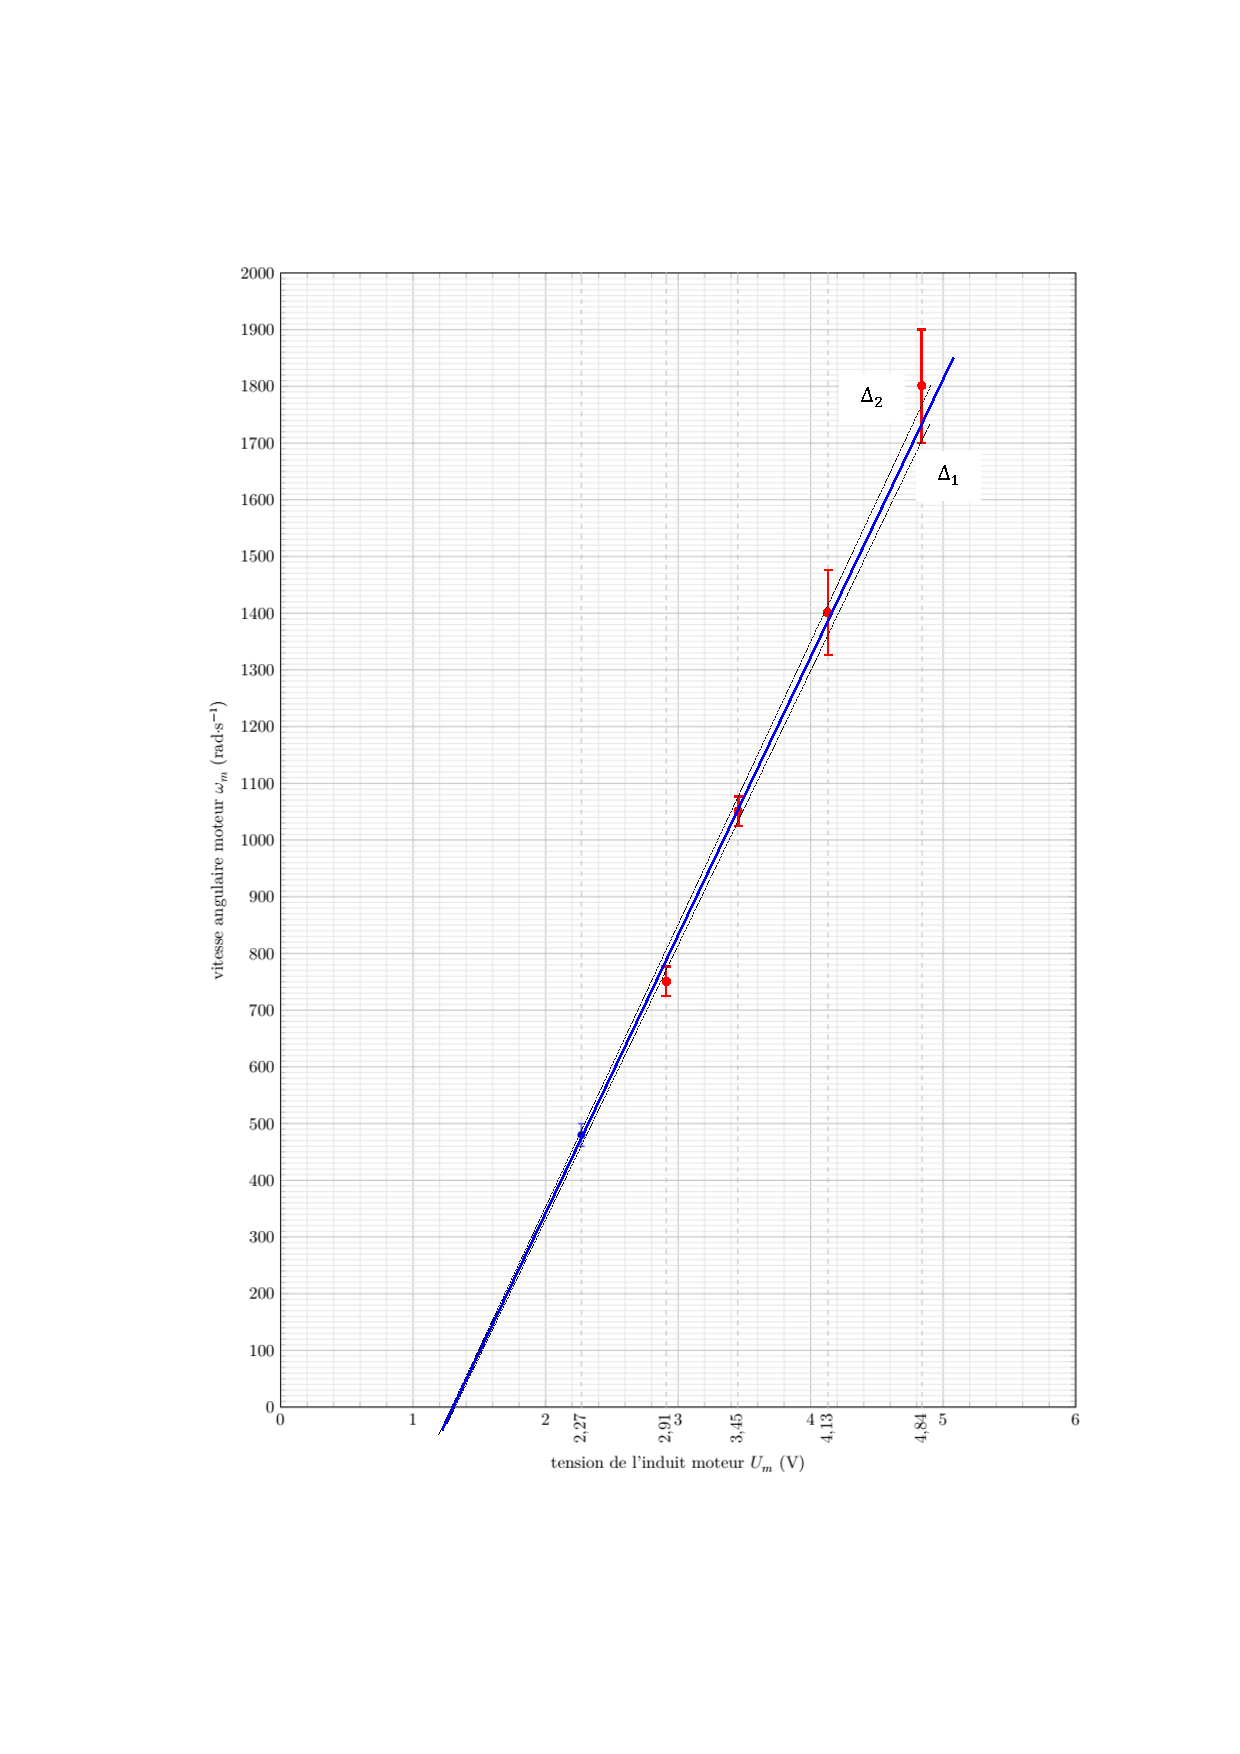
\includegraphics[width=1.0\textwidth]{images/courbe_dr_corrige.pdf}
\end{center}
}
{
\begin{center}
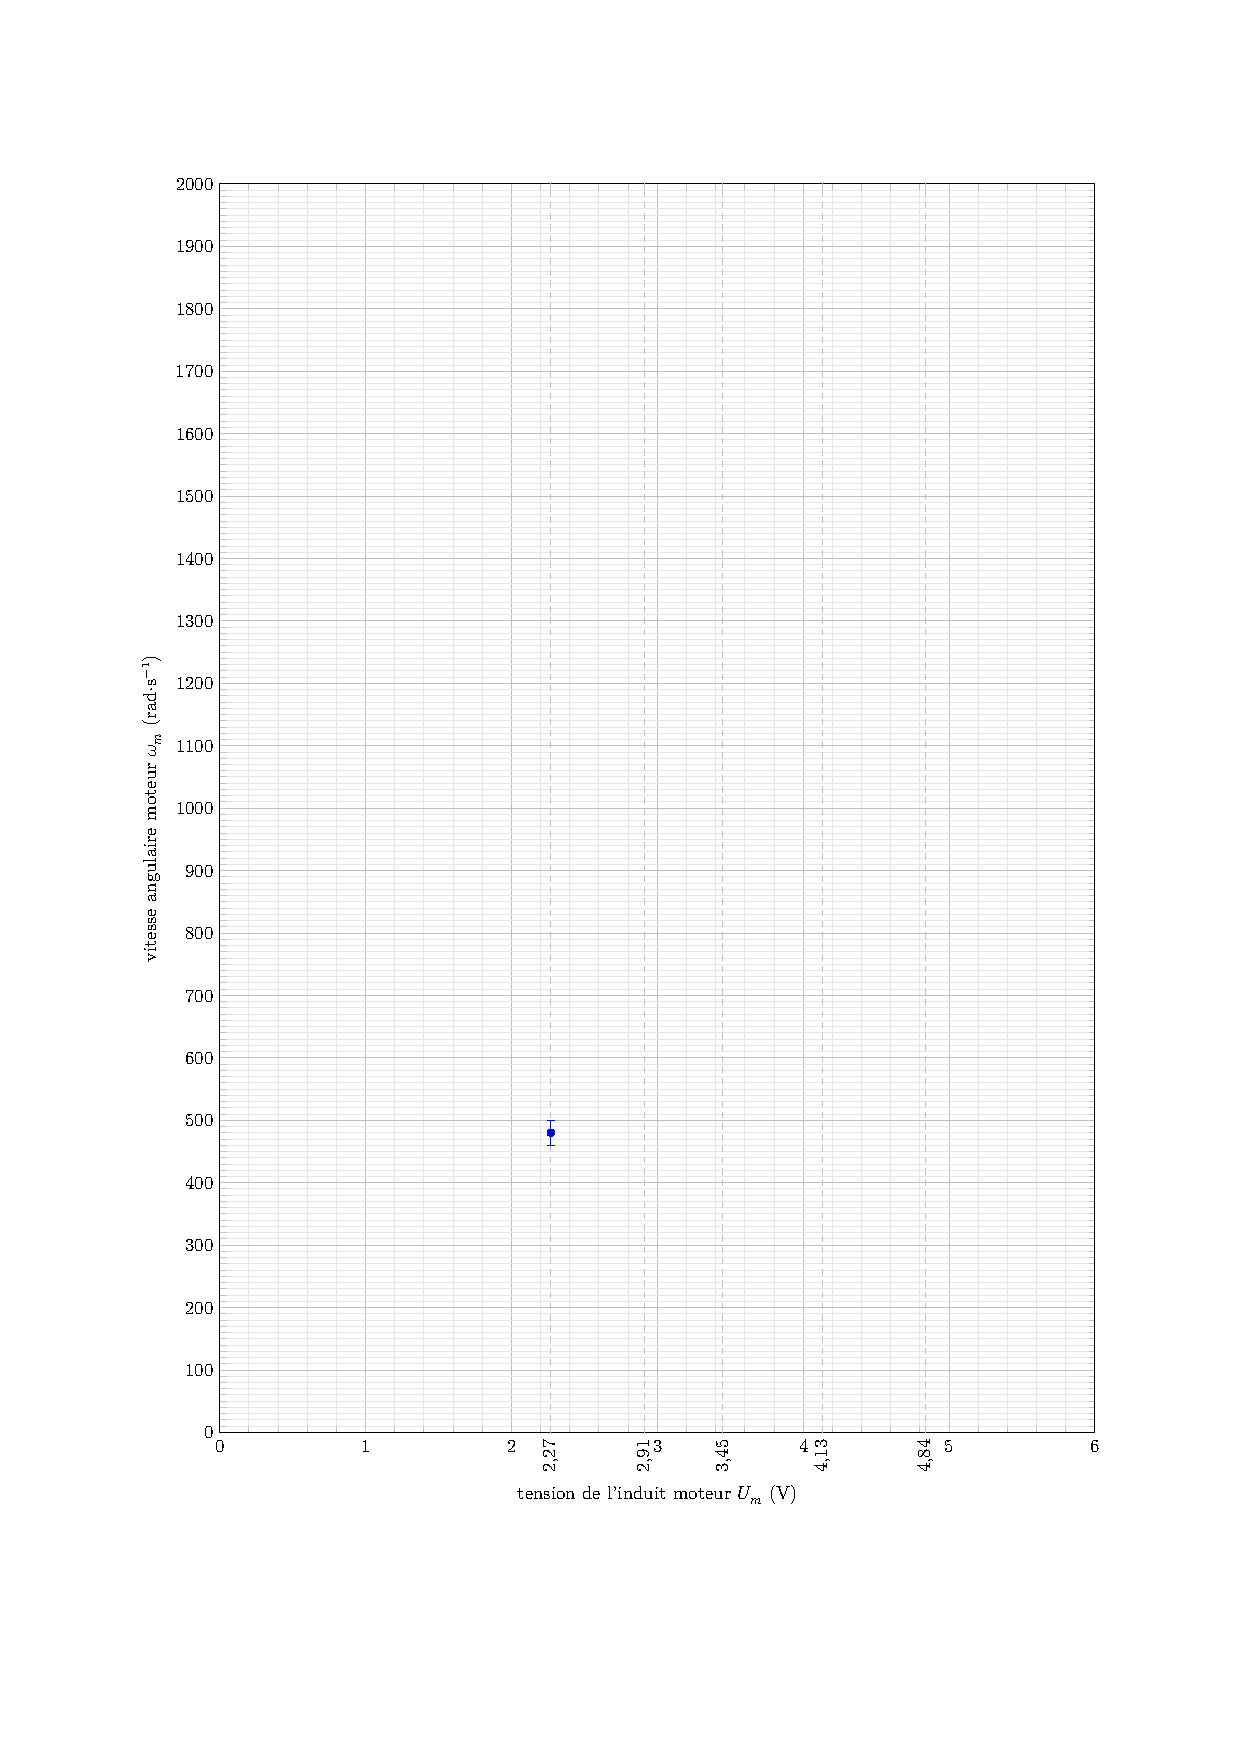
\includegraphics[width=1.0\textwidth]{images/courbe_dr.pdf}
\end{center}
}


\question{En déduire les valeurs numériques de $C_0$ et $f$.}

\begin{texteCache}
On a~: \(u_{m} = 1,3\ V\) en \(\omega_{m} = 0\ \frac{\text{rad}}{s}\)
 
Donc,

\[0 = 1,3K_{T} - R_{m}C_{0}\]

\[C_{0} = \frac{1,3K_{T}}{R_{m}} = 0,116\ mN.m\]

La pente de la droite tracée en question précédent vaut~:

\[\frac{K_{T}}{fR_{m} + K_{T}^{2}} = \frac{1730 - 0}{4,84 - 1,3} = 488\]

\[f = \frac{K_{T} - 488K_{T}^{2}}{488R_{m}} = 1,33 \bullet 10^{- 8}\ \frac{\text{N.m}}{\left( \frac{\text{rad}}{s} \right)}\]
\end{texteCache}

\question{Placer sur la courbe les incertitudes dues à la dispersion des mesures.}



\question{En tenant compte des incertitudes dans la mesure de vitesse, donner un encadrement de $C_0$ et de $f$.}

\begin{texteCache}

Très difficile de répondre à cette question. En effet, graphiquement,
  une seule droite passe par l'ensemble des intervalles de tolérance.

  Mais de façon un peu artificielle, on peut encadrer la courbe
  précédente par deux droites définies en pointillées sur le DR.

\begin{itemize}
\item
  \(C_{0,1} = 0,116\ mN.m\)~;
  \(f_{1} = 1,54 \bullet 10^{- 8}\ \frac{\text{N.m}}{\left( \frac{\text{rad}}{s} \right)}\)
\item
  \(C_{0,2} = 0,123\ mN.m\)~;
  \(f_{2} = 9,89 \bullet 10^{- 9}\ \frac{\text{N.m}}{\left( \frac{\text{rad}}{s} \right)}\)

  On pourrait donc encadrer les deux valeurs par~:
\end{itemize}

\[0,116 \bullet 10^{- 3} \leq C_{0} \leq 0,123 \bullet 10^{- 3}\ \]

\[9,89 \bullet 10^{- 9} \leq f \leq 1,54 \bullet 10^{- 8}\]

Avec cet encadrement, la tolérance sur le second point de mesure n'est
pas respectée.

\end{texteCache}

\question{On pose $\Omega_m(p)=H_u(p)\cdot U_m(p)+H_c(p)\cdot C_0(p)$. Exprimer $H_u(p)$ et $H_c(p)$ en fonction de $A$, $B$, $C$ et $D$.}

\begin{texteCache}
Par théorème de superposition : 
\begin{itemize}
\item \textbf{Détermination de $H_u(p)$ : } on prend $C_0(p)=0$ et $U_m(p)\neq 0$.
Par la formule de Black : 

\begin{align*}
H_u(p)=\dfrac{ABC}{1+ABCD}
\end{align*}
\item \textbf{Détermination de $H_c(p)$ : } on prend $C_0(p)\neq 0$ et $U_m(p)= 0$.
Par la formule de Black : 

\begin{align*}
H_u(p)=\dfrac{C}{1+ABCD}
\end{align*}
\end{itemize}
\end{texteCache}

\question{En utilisant le résultat de la question 9, montre que l'on peut mettre $H_u(p)$ et $H_c(p)$ sous la forme : 
\begin{align*}
\left\{
\begin{array}{l}
H_u(p)=\dfrac{K_m}{1+\dfrac{2\xi}{\omega_0}p+\dfrac{p^2}{\omega_0^2}}\\
\\
H_c(p)=\dfrac{K_c\left(1+\tau_m p\right)}{1+\dfrac{2\xi}{\omega_0}p+\dfrac{p^2}{\omega_0^2}}
\end{array}
\right.
\end{align*}
On donner les expression de $K_m$, $K_c$, $\tau_m$, $\xi$ et $\omega_0$ en fonctions des constantes du problème.
}

\begin{texteCache}
D'après la question 9 : 

\begin{align*}
A=\dfrac{1}{R_m+L_m\cdot p} \;;\; B=K_T\;;\;C=\dfrac{1}{J\cdot p+f}\;\text{et} \;D=K_e
\end{align*}

On obtient alors : 

\begin{align*}
H_u(p)=\dfrac{\dfrac{K_T}{\left(R_m+L_m\cdot p\right)\left(J\cdot p+f\right)}}{1+\dfrac{K_T\cdot K_e}{\left(R_m+L_m\cdot p\right)\left(J\cdot p+f\right)}}
=\dfrac{K_T}{\left(R_m+L_m\cdot p\right)\left(J\cdot p+f\right)+K_T\cdot K_e}\\
=\dfrac{\dfrac{K_T}{K_T\cdot K_e+R_m\cdot f}}{1+\dfrac{L_m\cdot f+J\cdot R_m}{K_T\cdot K_e+R_m\cdot f}p+\dfrac{J\cdot L_m}{K_T\cdot K_e+R_m\cdot f}p^2}
\end{align*}

On trouve alors $K_m=\dfrac{K_T}{K_T\cdot K_e+R_m\cdot f}$ ; $\omega_0=\sqrt{\dfrac{K_T\cdot K_e+R_m\cdot f}{J\cdot L_m}}$ et

\begin{align*}
\xi=\dfrac{\omega_0}{2}\dfrac{L_m\cdot f+J\cdot R_m}{K_T\cdot K_e+R_m\cdot f}=\dfrac{1}{2}\sqrt{\dfrac{K_T\cdot K_e+R_m\cdot f}{J\cdot L_m}}\dfrac{L_m\cdot f+J\cdot R_m}{K_T\cdot K_e+R_m\cdot f}\\
\xi=\dfrac{1}{2}\dfrac{L_m\cdot f+J\cdot R_m}{\sqrt{\left(K_T\cdot K_e+R_m\cdot f\right)J\cdot L_m}}
\end{align*}

\begin{align*}
H_c(p)=\dfrac{\dfrac{1}{J\cdot p+f}}{1+\dfrac{K_T\cdot K_e}{\left(R_m+L_m\cdot p\right)\left(J\cdot p+f\right)}}
=\dfrac{R_m+L_m\cdot p}{\left(R_m+L_m\cdot p\right)\left(J\cdot p+f\right)+K_T\cdot K_e}\\
=\dfrac{R_m}{K_T\cdot K_e+R_m\cdot f}\dfrac{1+\dfrac{L_m}{K_T\cdot K_e+R_m\cdot f}p}{1+\dfrac{L_m\cdot f+J\cdot R_m}{K_T\cdot K_e+R_m\cdot f}p+\dfrac{J\cdot L_m}{K_T\cdot K_e+R_m\cdot f}p^2}
\end{align*}

On trouve donc $\tau_m=\dfrac{L_m}{R_m}$ et $K_c=\dfrac{R_m}{K_T\cdot K_e+R_m\cdot f}$


\end{texteCache}

\question{Déterminer l'expression de la fonction de transfert $E$.}

\begin{texteCache}
$\omega_m(t)=\dfrac{d\theta_m(t)}{dt}$ ainsi $\Omega_m(p)=p\cdot \theta_m(p)$, d'où $E=\dfrac{1}{p}$

\end{texteCache}

\question{Donner l'expression du gain d'adaptation $K_a$ en fonction des grandeurs définies dans le schéma bloc (figure\ref{fig14}) pour que le système soit correctement asservi.}

\begin{texteCache}
Pour que le système soit correctement asservi, il faut vérifier : 

\begin{align*}
\varepsilon(p)=0\Leftrightarrow D_c(p)=D_c(p).
\end{align*}

Or,

\begin{align*}
\varepsilon(p)=K_a\cdot D_c(p)-\dfrac{K_{cod}K_{pc}}{K_{cin}}D_l(p)
\end{align*}

On obtient alors : 

\begin{align*}
\boxed{
K_a=\dfrac{K_{cod}K_{pc}}{K_{cin}}
}
\end{align*}
\end{texteCache}

\question{Donner l'expression de $\varepsilon(p)$ en fonction de $D_c(p)$ et des constantes $K_a$, $K_{cin}$, $K_m$, $\xi$ et $\omega_0$.}

\begin{texteCache}
\begin{align*}
\varepsilon(p)=K_a\cdot \left(D_c(p)-D_l(p)\right)=K_a\cdot \left[D_c(p)-\frac{K_{cin}}{p}H_u(p)\cdot K_p\cdot \varepsilon(p)\right]
\end{align*}

On obtient donc : 

\begin{align*}
\boxed{
\varepsilon(p)=\dfrac{K_a}{1+\frac{K_{cin}\cdot K_p}{p}H_u(p)}\cdot D_c(p)=\dfrac{K_a}{1+\frac{K_{cin}\cdot K_p\cdot K_m}{p\left(1+\dfrac{2\xi}{\omega_0}p+\dfrac{p^2}{\omega_0^2}\right)}}\cdot D_c(p)
}
\end{align*}

\end{texteCache}

\question{En déduire l'erreur statique théorique issue de la modélisation et conclure vis-à-vis du cahier des charges.}

\begin{texteCache}

Pour déterminer l'erreur statique $\varepsilon_s$ on pose $D_c(p)=\frac{D_0}{p}$.

On calcule alors $\varepsilon_s=\lim_{t\rightarrow+\infty} \varepsilon(t) = \lim_{p\rightarrow0} p\;\varepsilon(p).$

On obtient donc : 

\begin{align*}
\lim_{p\rightarrow0} p\;\varepsilon(p)=\dfrac{p\cdot K_a}{1+\frac{K_{cin}\cdot K_p\cdot K_m}{p\left(1+\dfrac{2\xi}{\omega_0}p+\dfrac{p^2}{\omega_0^2}\right)}}\cdot\frac{D_0}{p}=0
\end{align*}

Le cahier des charges est bien respecté.

\end{texteCache}


\question{Conclure sur l'étude en indiquant :
\begin{itemize}
\item les critères du cahier des charges qui sont validés avec les valeurs ;
\item les hypothèses ;
\item les sources des écarts observés entre le comportement simulé, souhaité et réel de l'objectif photographique ;
\end{itemize}
}

\begin{texteCache}
\begin{itemize}
\item
  \textbf{Critères du cahier des charges~:}

  \begin{itemize}
  \item
    Erreur statique~: la courbe de la réponse indicielle semble avoir
    une asymptote à 2 mm en \(t \rightarrow \infty\) malgré l'indication
    de 1,994 mm~; l'erreur statique serait donc nulle et le critère
    respecté.
  \item
    Rapidité~: \(t_{r5\%} = 0,13\ s < 0,6\ s\) donc critère respecté.
  \item
    Aucun dépassement~: critère respecté.
  \end{itemize}
\item
  \textbf{Hypothèses~:}

  \begin{itemize}
  \item
    Le modèle cinématique ne prend pas en compte les éventuels jeux dans
    la transmission, l'éventuel glissement de la courroie et son
    élasticité.
  \item
    Les masses et inerties de certains solides sont négligées pour le
    calcul de l'inertie équivalente.
  \item
    On fait l'hypothèse que le moteur est alimenté en courant continu
    alors qu'il est vraisemblablement alimenté par un hacheur.
  \item
    On considère un modèle couple de frottement sec constant.
  \end{itemize}
\item
  \textbf{Ecarts~:} les courbes de réponses indicielles simulée et réelle sont
  très proches, il est difficile de statuer sur les écarts. Les jeux
  dans la transmission pourraient expliquer le retard sur la réponse
  indicielle mesurée. Cependant, les autres causes d'écarts pourraient
  être~:

  \begin{itemize}
  \item
    L'estimation de \(K_{e},C_{0}\) et \(f\) est faite à partir de
    grandeurs entachées d'erreurs de mesure et de la chaîne
    d'acquisition notamment le filtrage numérique qui peut induire un
    retard et une erreur due à la discrétisation.
  \item
    La stabilité du système n'est vérifiée que sur le modèle linéarisé.
  \item
    Le correcteur utilisé réellement est vraisemblablement un correcteur
    numérique.
  \item
    Il existe des modèles de frottement plus complexes que celui choisi.
  \end{itemize}
\end{itemize}

\end{texteCache}





